\section{Powering the Device}
Our team plans to power our raspberry pi using solar power. The components we will use to do so can be found below. 
\begin{itemize}
    \item Lithium Polymer Charger
    \item Lithium Ion polymer Battery
    \item Powerboost 500
    \item Solar Panel
\end{itemize}

The Li/Poly charger would connect to the 2W, 6V solar panel. The charger has the charge current of 500 mA, but can be adjusted to anywhere in between 100 mA and 1000 mA by soldering a resistor. Charging is performed in three stages: first a preconditioning charge, then a constant-current fast charge and finally a constant-voltage trickle charge to keep the battery topped-up. The Charger is connected to a Li/Poly battery. This battery has a capacity of 2500mAh for a total of about 10 Wh, and the output ranges from 4.2V when completely charged to 3.7V. One of the outlets of the charger will be connected to the Powerboost 500 component. This little DC/DC boost converter module can be powered by any 3.7V LiIon/LiPoly battery, and convert the battery output to 5.2V DC, to run the Raspberry Pi. This hardware configuration can be seen in Figure \ref{flow} below. \hfill

\begin{figure}[H]
\centering
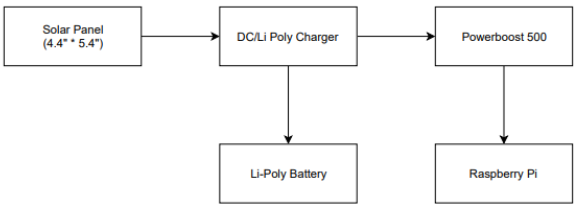
\includegraphics[scale=0.8]{graphics/power_flow.PNG}
\caption{Power Flow Chart}
\label{flow}

\end{figure}